%% LaTeX template for BSc Computing for Games final year project dissertations
%% by Edward Powley
%% Games Academy, Falmouth University, UK

%% Based on:
%% bare_jrnl.tex
%% V1.4b
%% 2015/08/26
%% by Michael Shell
%% see http://www.michaelshell.org/
%% for current contact information.
%%
%% This is a skeleton file demonstrating the use of IEEEtran.cls
%% (requires IEEEtran.cls version 1.8b or later) with an IEEE
%% journal paper.
%%
%% Support sites:
%% http://www.michaelshell.org/tex/ieeetran/
%% http://www.ctan.org/pkg/ieeetran
%% and
%% http://www.ieee.org/

%%*************************************************************************
%% Legal Notice:
%% This code is offered as-is without any warranty either expressed or
%% implied; without even the implied warranty of MERCHANTABILITY or
%% FITNESS FOR A PARTICULAR PURPOSE! 
%% User assumes all risk.
%% In no event shall the IEEE or any contributor to this code be liable for
%% any damages or losses, including, but not limited to, incidental,
%% consequential, or any other damages, resulting from the use or misuse
%% of any information contained here.
%%
%% All comments are the opinions of their respective authors and are not
%% necessarily endorsed by the IEEE.
%%
%% This work is distributed under the LaTeX Project Public License (LPPL)
%% ( http://www.latex-project.org/ ) version 1.3, and may be freely used,
%% distributed and modified. A copy of the LPPL, version 1.3, is included
%% in the base LaTeX documentation of all distributions of LaTeX released
%% 2003/12/01 or later.
%% Retain all contribution notices and credits.
%% ** Modified files should be clearly indicated as such, including  **
%% ** renaming them and changing author support contact information. **
%%*************************************************************************


\documentclass[journal]{IEEEtran}

\usepackage{graphicx}
% Insert additional usepackage commands here
\usepackage[hyphens]{url} % <===========================================
\usepackage[hidelinks]{hyperref} % Allows clickable reference lists
\usepackage[none]{hyphenat} %Stops breaking up words in table
\usepackage{cite}
\usepackage{listings}
\usepackage{amssymb}
\usepackage{upgreek}
\usepackage{siunitx}

\usepackage[table,pdftex,dvipsnames]{xcolor} 

\begin{document}
%
% paper title
% Titles are generally capitalized except for words such as a, an, and, as,
% at, but, by, for, in, nor, of, on, or, the, to and up, which are usually
% not capitalized unless they are the first or last word of the title.
% Linebreaks \\ can be used within to get better formatting as desired.
% Do not put math or special symbols in the title.
\title{ How Will a Mixed-Initiative Level Editor that Predicts User Requirements Affect the Levels Created?}
%
%
% author name

\author{Tristan Barlow-Griffin - 1607804}

% The paper headers -- please do not change these, but uncomment one of them as appropriate
% Uncomment this one for COMP320
%\markboth{COMP360: Research }{COMP320: Research Review and Proposal}
% Uncomment this one for COMP360
\markboth{COMP360: Dissertation}{COMP360: Dissertation}

% make the title area
\maketitle

% As a general rule, do not put math, special symbols or citations
% in the abstract or keywords.
\begin{abstract}
Mixed-initiative (MI) systems are becoming more common both in and outside of the games industry. These MI systems are taking an ever-increasing number of roles. These roles range from generating entire levels, to fostering creativity in game designers. With the increasing cost of game development, having a tool that can help to quickly and effectively prototype levels will reduce the costs of development significantly.
This paper explores some of the effects that introducing an MI component may have to a level editor. To identify what effects to look for, this paper uses existing research into predictive texting and MI level editors. From this research, five hypotheses are proposed. To test the hypotheses, this paper proposes an experiment where the same group of users create different levels with and without the MI present. The results demonstrate the benefits and drawbacks of using an MI level editor and provide direction for improvement.
\end{abstract}

\section{Introduction} \label{intro}
\IEEEPARstart{T}{his} research project looks into how a prototyping tool with a Mixed-Initiative (MI) component that predicts user requirements will affect the process and design of a level. A prototype is the initial design of an object \cite{prototype}, the prototyping phase is used to quickly test certain aspects of a products' design so the designer can identify and solve any problems before full production commences\cite{budde1992prototyping}. Fullerton \textit{et all} \cite[p.~150]{fullerton2004game} state there are two kinds of prototyping in games: Physical and Software prototypes. Since the publication of Fullerton's\textit{et al}\cite{fullerton2004game} book in 2004, the accessibility of tools that help designers prototype levels has increased. Fullerton \textit{et al} \cite[p.~164]{fullerton2004game} also describes a level editor as a good way to prototype levels. The free to download game engine called \textit{Unreal Engine 4} (UE4) has a level editor built into it. Within this editor, the designers can create basic geometry scaling them to fit their needs. In addition, designers can add custom meshes and programmable objects to turn their levels into games.

The prototyping phase is meant to test the design of a product, the less time and resources required to produce an artefact that can demonstrate the proposed design, the better. It could be argued the less time a designer puts into a particular design the less attached to the design they become. When collaborating in a group, differing opinions can cause different constraints to be set on the design of a product. While a given design may satisfy the original designers set constraints, the prototype may have to be discarded as it did not meet the other requirements set by the team. Identifying and discarding concepts early in development can save a lot of time and energy \cite[p.489]{stempfle1999thinking}. Arguably, this will reduce the negative impacts to interpersonal relations that idea dismissal may have.

In this paper, we propose a level editor that is meant to only prototype a levels' design. This will allow for less focus on the polish of the level created as the aim of the prototype is just to test if it fits the users' requirements. This paper will build upon a standard level editor by adding an MI component. The component implements features requested from Alvarez \textit{et al}\cite{alvarez2018fostering} study on their MI level editor. The implementation of these features is meant to increase the overall ease of designing a level by predicting what the user may require. In addition, this paper looks at the Sentient Sketchpad\cite{liapis2013sentient} an existing MI level editor, comparing their design to MI tool design theory and general user interface (UI) design theory. The hypotheses in this paper are only concerned with how the MI component interacts with the participants and what kind of impact the interactions will have when trying to prototype a level. Looking at existing studies on the most effective prediction methods \cite{shepperd2001comparing,mendes2002further, wen2012systematic} this paper identifies and evaluates the methods proposed in the context of an MI level editor.

\section{Related Work}
The lack of documentation about prediction methods being used in game design required this paper to go beyond the scope of just game design examples. The methods of prediction used in this study must be effective for the hypotheses to be tested accurately. To this end, Section~\ref{prediction} looks at currently used prediction methods comparing the performance results of each method. In Section~\ref{MI}, MI tools are grouped into two broad categories using Liapis~\textit{et al}\cite{liapis2016mixed} definition. The definition of MI used in this paper will also be defined in Section~\ref{MI}. Defining these groups makes it easier to distinguish between the most common types of MI tools. This section will also explore the different ways MI tools are being leveraged both within and outside of the games industry. In Section~\ref{UI} there is an evaluation of the existing MI level editors. Section~\ref{UI} also contains a discussion and comparison of these MI editors in the context of more general MI and UI design theory.

\section{Mixed-initiative} \label{MI}
The term mixed-initiative was first introduced in \textit{1970} by Jaime R \cite{carbonell1970mixed}.
It describes a process whereby a computer and a human designer work together to achieve a goal. Other definitions of MI build on the idea of human-computer co-creativity. This paper will use the first definition of MI presented, as trying to define creativity is a very complex matter in itself. 

There are two broad categories that MI tools can be grouped into, Interactive evolution and Computer-aided design \cite{liapis2016mixed}. 
\begin{itemize}
    \item \textit{Interactive evolution}(IE) is where the designer has the idea, and the computer helps them realise it. The computers' role is to evaluate the humans' design, presenting alternative solutions if any constraints are broken. 
    
    \item \textit{Computer-aided design} (CAD) is where the computer generates the content, but does not evaluate the quality of the produced work. In CAD, the human designer will evaluate the work and use these evaluations to move towards a more desirable product space.
\end{itemize}

The first documented MI tool created helped students to learn the English language\cite{carbonell1970mixed}. The uses of MI tools have greatly expanded since 1970 and have been described as a backbone tool for designers \cite{alvarez2018fostering}. The application of MI systems in more complex environments have given mixed results \cite{barnes2015designing}. Barnes \textit{et al}\cite{barnes2015designing} found that in most cases, systems that divide decision making between a human and an intelligent agent were generally more effective than if decisions were just dependent on the one. This can be seen with predictive texting. Only choosing the words suggested to you by your phone can result in unexpected and hilarious results \cite{quicktype}. Barnes \textit{et al}\cite{barnes2015designing} found that human designers were better at making abstract decisions and inferring the significance of an object or event. Kantosalo \textit{et al}\cite{kantosalo2014isolation} focus their MI tool on user-centred design, this means their AI agent had less responsibility than the human user. Kantosalo \textit{et al}\cite{kantosalo2014isolation} propose future work where the agent and the designer have an equal role in the system, they do not make any conjecture on the anticipated results.

Procedural content generation(PCG) and CAD are closely related fields, the difference between CAD and PCG is in the evaluation period. If a designer were to use a PCG algorithm to generate a level and then look through the produced results, evaluating and picking maps this would be considered CAD\cite{liapis2016mixed}. For it not to be considered CAD, the PCG algorithm would have to perform the evaluation itself. For example, this might include checking if the map is completable or if it is a certain size. The field of PCG has advanced significantly in recent years \cite{van2013designing}. The uses of PCG are ever increasing as publishers seek to lower costs of production\cite{doherty2005mixed, font2016constrained}.

One may choose to use PCG in games as it will increase the quantity and variation of levels produced ensuring replayability \cite{karavolos2015mixed}. PCG algorithms can also be shipped with the games they are made for, this allows for an inexhaustible source of new maps \cite{johnson2010cellular}. Doing so will extend the games life-span giving the players an amount of content that would otherwise be impossible. Although there is no guarantee that this content will be interesting or unique. However, using CAD tools to generate maps there will always require a human element to evaluate the maps. With this input the human designer may discard maps that are similar to existing maps, thus providing quality assurance not present in a PCG algorithm.

Prototyping a level should be a fast iterative process \cite{smith2011tanagra}, the method used to prototype should allow for instant feedback on the design. This feedback needs to have an easy channel back to the designer so that amendments can be made easily. Map generation algorithms, even in under ideal circumstances will only provide the designer with a set of parameters to change\cite{doran2010controlled}. Small variations in the given parameters can produce large changes in the maps design\cite{regier2009random}. This will make it difficult to make small changes when given feedback. As a result, this reduces the effectiveness of a CAD approach when trying to prototype levels.

Within an IE environment, the core of the creative process relies on the human designer. As the main creative driver, the human has the most input. Ideally, the computer will add value by providing supplementary support, for example, alerting the designer when constraints have been broken. It can be argued as the constraints are determined more by the human, the size of the possible output space will be larger. Yanakakis \textit{et al} \cite{yannakakis2014mixed} claim that CAD examples like PCG limit the designers' intentions as they follow their own algorithms. Doran and Parberry\cite{doran2010controlled} inadvertently corroborate Yanakaki\textit{et al}\cite{yannakakis2014mixed} view, as they say, a PCG algorithm should ideally, have a set of designer-centric parameters as their only form of control. This limited control over the creation of levels may, in some situations, be enough. The user requirements of a map change most often during the prototyping phase. The level of control provided through CAD might not be enough to handle the necessary changes. 

\section{Mixed-Initiative Level Editors } \label{UI}
A user interface should be intuitive to use and not require any additional helping systems \cite{oppermann2002user}. Liapis \textit{et al} \cite{liapis2013sentient} aim to achieve this by creating a design tool that allows users to create levels using a low-resolution graphical interface. Figure~\ref{Sketchbook} shows the interface used to design levels for a strategy game. The designer can place tiles on the map which will colour in the given tile with the placed tiles colour. During a tile placement, the tool will test for the playability of the map, checking to see if placing the current tile will break any of the games' constraints. The Sentient sketchbook also provides alternative viewing modes, examples of the viewing modes can be seen in Figure~\ref{Sketchbook2}. There is no mention in the study how frequently these tools were used, Galtiz \cite[p.~752]{galitz2007essential} warns against too many graphics on the screen.

\begin{figure}[h]
	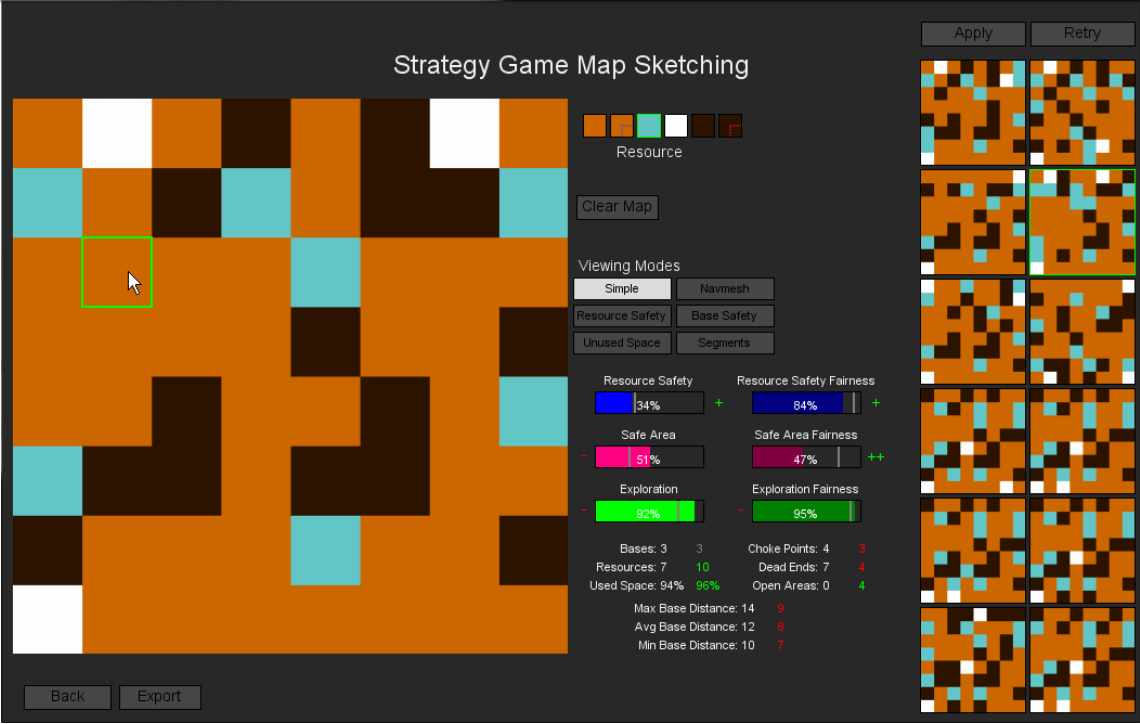
\includegraphics[width=1.0\linewidth]{SentientSketchbook.PNG}
	\caption{Liapis \textit{et al} Sentient Sketchbook during a design session ~\cite{liapis2013sentient}.}
	\label{Sketchbook}
\end{figure} 

\begin{figure}[h]
	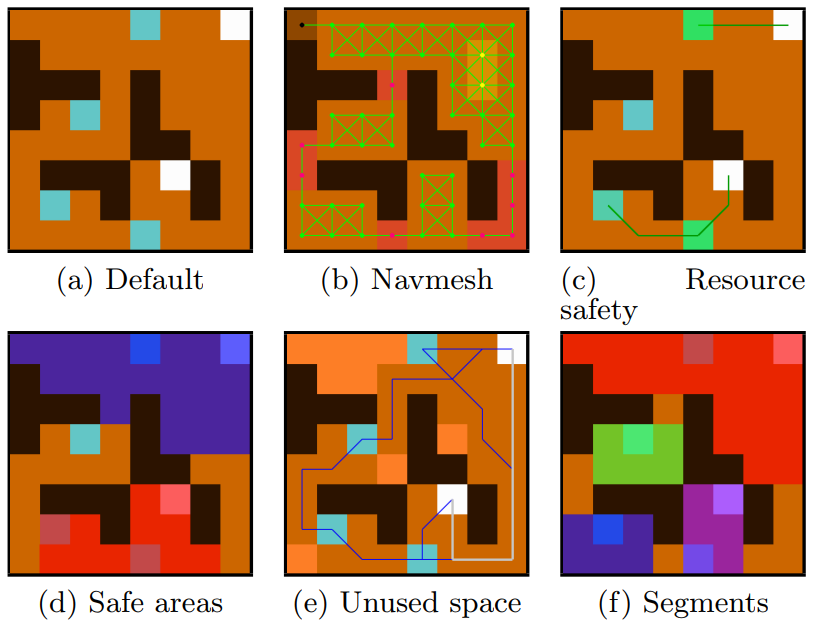
\includegraphics[width=1.0\linewidth]{SentientSketchbook2.PNG}
	\caption{Liapis \textit{et al} Sentient Sketchbook Different viewing modes ~\cite{liapis2013sentient}.}
	\label{Sketchbook2}
\end{figure} 

Baldwin \textit{et al} \cite{baldwin2017mixed} have also implemented an MI dungeon designer called the evolutionary dungeon designer or (EDD) for short. EDD is closer to a CAD tool than the IE tool Sentient Sketchbook \cite{liapis2013sentient}. While the approaches may be different see Figure~\ref{EDD}, both MI tools allow for large customisation of the levels generated see Figure~\ref{EDD}. Baldwin \textit{et al} \cite{baldwin2017mixed} take a different approach to Liapis \textit{et al}\cite{liapis2013sentient}. Baldwin \textit{et al} \cite{baldwin2017mixed} core concept is to identify design patterns within the level design. These design patterns consist of multiple tiles that constitute common patterns found in games. Alvarez \textit{et al}\cite{alvarez2018fostering} builds upon the EDD suggested in \cite{baldwin2017mixed} by adding an IE element to it. It could be argued that the new version of the EDD has an improved interface with a reduction in excess drop-down menus, see Figure~\ref{EDD2}. Beyond the aesthetic differences, Alvarez \textit{et al}\cite{alvarez2018fostering} dungeon designer integrates key aspects of the Sentient Sketchpad \cite{liapis2013sentient}. The second edition of the EDD allows the user to design their own levels, it will then offer suggestions based upon the map the user created, this can be seen in the top right corner of figure~\ref{EDD2}. The results from Alvarez \textit{et al}\cite{alvarez2018fostering} experiment focused on whether their tool fostered creativity in the participants using it. Included with the results is a table of requested features made by the participants of the study. One key element highlighted is that the EDD should do a ``bit more automated assistance when doing manual designs, which can reduce clicking around the program" \cite[Table 2]{alvarez2018fostering}. Another significant feature request was for the dungeon designer to take into account the pattern of the entire dungeon, using the map of the dungeon to generate new rooms.

\begin{figure}[h]
	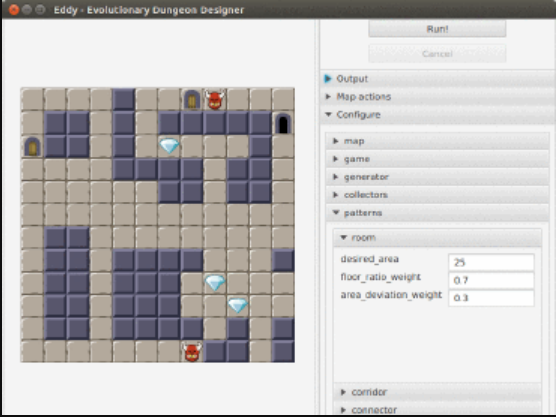
\includegraphics[width=1.0\linewidth]{EDD.PNG}
	\caption{ Baldwin \textit{et al} Evolutionary Dungeon Designer user interface ~\cite{baldwin2017mixed}.}
	\label{EDD}
\end{figure} 

\begin{figure}[h]
	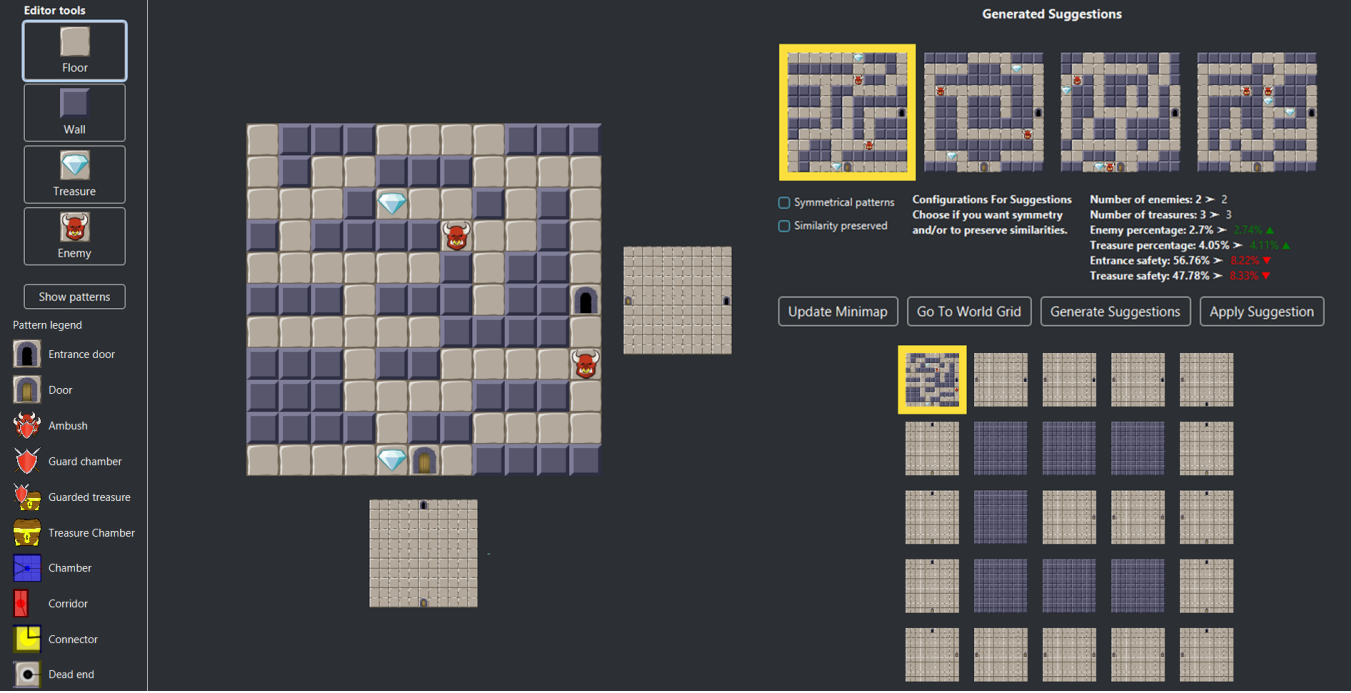
\includegraphics[width=1.0\linewidth]{EDD2.PNG}
	\caption{ Alvarez \textit{et al} Evolutionary Dungeon Designer with modifications user interface ~\cite{alvarez2018fostering}.}
	\label{EDD2}
\end{figure} 

Horvitz \cite{horvitz1999principles} proposes 12 critical factors to take into consideration when making an MI user interface. While Horvitz \cite{horvitz1999principles} focuses on an MI assistant for Microsoft Outlook (emailing software) it can be argued that some of these factors are relevant for a level designer. The first factor that is listed is that an MI tool needs to add significant value through the automation of services. An example of a service automated by emailing assistant is the sorting of a users' emails into different categories. Within the context of \cite{liapis2013sentient} they satisfy \cite{horvitz1999principles} first critical factor by allowing the computer to automate some of the map design services like checking for broken game constraints. Liapis \textit{et al} \cite{liapis2013sentient} also allows their algorithm to take on a creative role all be it based on an original human designed map. Within this project, the focus will not be on the creative aspect as the definition of creativity is hard to for a computer to understand \cite{jordanous2010defining}. Alvarez \textit{et al}\cite{alvarez2018fostering} found their MI tool is better at providing controllability than expressivity, when the user imposes their vision, as it is hard for a computer to capture the designers' vision. It can be argued that an MI tool could not consistently add value if it cannot capture the designers' vision. Smith \textit{et al}\cite{smith2011tanagra} believe that human designers strengths lay in creativity and their ability to evaluate good content and which the computer lacks. 

Another factor raised by Horvitz \cite{horvitz1999principles} is that a tool must consider minimizing the costs of poor guesses about the users' goals. Even with an extensive history of the users' requirements, novel use of the tool might be required. It is important for a system to recognise when something novel is happening and for it not to attempt predictions. Some authors find value in these missed guesses and even seek to find novelty search spaces \cite{liapis2013sentient}. Other authors \cite{liapis2016can,alvarez2018fostering, yannakakis2014mixed} claim these kinds of mistakes can foster creativity and alternate suggestions that do not aim to predict the user can be beneficial. On the right-hand side of Figure~\ref{Sketchbook} the results of the guessing algorithm are shown. Clicking retry will remove the current maps and create new ones for the designer to evaluate.

None of the above examples \cite{alvarez2018fostering, liapis2013sentient, baldwin2017mixed} satisfy Barnes \textit{et al}\cite{barnes2015designing} statement that an MI systems UI must provide transparency to the reasoning behind the agents' actions. In all cases given above\cite{alvarez2018fostering, liapis2013sentient, baldwin2017mixed} , when generating new suggestions the reasoning behind each suggestion was not given to the designer. The designer is presented with the statistics of the current map generated (density, number of resources etc.) but it is not clear from the interface how these statistics are being used. Lee and See\cite{lee2004trust} agrees with Barnes \textit{et al}\cite{barnes2015designing} that MI systems should be transparent, they go so far as to say it is required for a human to trust the automation process \cite{lee2004trust}.

\section{Prediction Methods} \label{prediction}
Predictive texting increases the average message length users send to each other \cite{ling2005length} as well as the speed the words are written \cite{dunlop2000predictive}. The same theory may apply to game design. If patterns of a users game design are established, an AI system may be able to assist in design. In this section, this paper will look into different methods of predicting human requirements, this paper will also discuss the pros and cons of each technique.

The researchers of \cite{chipalkatty2013less} have tested alternate methods for predicting human input so as to abstract the low-level movements of the robots the humans were controlling. They built on the idea that humans are good for high-level abstract tasks, but an AI agent was much better at performing low-level repetitive control tasks. In addition, they found that when trying to predict the next human input, trying to identify patterns in a history of events was not successful. Instead, using just the last event yielded much better results, hence their title ``less is more". Instead of using current human inputs, \cite{bhatia2016targeted} used the history of the users' social media page to predict the users' interests. Perhaps if the authors of \cite{chipalkatty2013less} had looked less at the input history of the human and instead focused on grouping inputs together to create larger actions. Similar, to how modern day phones often predict entire sentences rather than just single words.

\subsection{Markov Chains}
Markov Chains implements a theory similar to the methods previously discussed by Bhatia and Hasija \cite{bhatia2016targeted}. A Markov chain is a special kind of process that works under the assumption that the state at time \textit{t+1} depends only on the current state. Another explanation is the state at time \textit{t+1} is exclusively dependent on the state at time \textit{t}. This means State \textit{t+1} is not dependent on the history of the states leading up to it\cite{ye2000markov}. This technique has been proven useful for predicting anomalies in systems \cite{ju2001hybrid, gwadera2005markov, ye2000markov} where the states are heavily dependent on the latter state happening. However, it is hard to see how during a creative process, where the next state is dependent on the vision of the designer, the state at \textit{t+1} can be predicted from just knowing the state at \textit{t}. 
The introduction of a Markov model makes Markov Chains method more viable as a prediction technique. A Markov model can be used to describe the probabilistic relationship between the previous states in a Markov Chain\cite{markov1971extension}. Higher order Markov chains relax the rule of the next state being only dependent on the current state by allowing the network structure to look \textit{n} number of states back from the current state\cite{ching2008higher}. Snodgrass and Ontanon\cite{snodgrass2017learning} used Markov models as a way to model level data. Using these Markov models Snodgrass \textit{et al}\cite{snodgrass2017learning} applied different sampling techniques, they found using their higher order Markov chains to be more effective than using standard Markov chains. This conflicts with Chipalkatty \textit{et al}\cite{chipalkatty2013less} findings of ``less is more", Snodgrass and Ontanon\cite{snodgrass2017learning} found that using a history of states to predict the next state was more effective to achieve their goals.

\subsection{Artifical Neural Network}
An artificial neural network (ANN) consists of many nodes that are divided into separate layers. Each node receives inputs from other nodes, the value of these inputs depends on the weight of the connection between the nodes \cite{lai2010prediction}. ANN are used in prediction methods focusing on outputting numerical values \cite{lai2010prediction, akdag2009estimation}. Shepperd and Kadoda \cite{shepperd2001comparing} found that case-based reasoning(CBR) outperformed an ANN. However, Shepperd and Kadoda\cite{shepperd2001comparing} highlighted the dependence of the respective techniques on the nature of the training sets used. Figure~\ref{learningSets} shows stepwise regression procedure (SWR) proving to be more accurate at prediction than both CBR and ANN on small datasets. A time series approach to neural networks has been found to increase their accuracy when dealing with world state predictions \cite{hazarika1998neural}. The number of data points in the training set that Hazarika and Lowe\cite{hazarika1998neural} used was much larger than in \cite{shepperd2001comparing} at 500 points for training and 250 for validation. Looking at examples from \cite{liapis2013sentient, alvarez2018fostering,  baldwin2017mixed} the maximum level dimensions are 12 tiles wide by 12 tiles tall. This means that the maximum number of data points provided by one map would be 124, which is far less than Hazarika and Lowe\cite{hazarika1998neural} use to train their ANN.

\begin{figure}[h]
	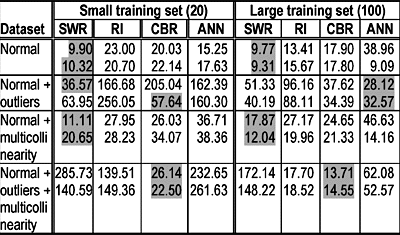
\includegraphics[width=1.0\linewidth]{trainingSets.PNG}
	\caption{Shepperd \textit{et al} Analysis of Accuracy (MMRE) for Continuous Model (Y1) ~\cite{shepperd2001comparing}.}
	\label{learningSets}
\end{figure} 

\subsection{Case-based Reasoning and Stepwise Regression procedure}
Case-based reasoning (CBR) is a prediction technique that uses a history of completed products to predict solutions to problems in the current product. This is done by comparing features in the current problem description to problems already solved in existing projects. Usually, the problem description that is most similar to the current problem is used to estimate the solution\cite{watson1998applying, mendes2002further}. The core of a case-based reasoner is solving new problems by using or adapting solutions from old problems \cite[p. 1]{riesbeck2013inside}. Watson \cite{watson1999case} describes CBR as a methodology, not a technique and provides several different techniques to apply CBR. Mendes and Mosley\cite{mendes2002further} have compared some of the techniques found in \cite{watson1999case} as well as additional techniques. They found that using a CBR technique that used adaptation rules performed significantly better than techniques that did not use adaption rules. In addition, they found the CBR techniques that used weighted Euclidean distance also gave the best predictions. Much like Shepperd and Kadoda\cite{shepperd2001comparing}, Mendes and Mosely\cite{mendes2002further} also found that SWR gave the best prediction accuracy ``for all measures of prediction accuracy'' \cite[p. 11]{mendes2002further}. The dataset used in \cite{mendes2002further} consisted of 34 data points which could be considered a small data set when comparing the number of data points used in \cite{hazarika1998neural}. Looking at Figure~\ref{learningSets}  there is a strong case for both SWR and CBR as prediction techniques with small data sets. Wen \textit{et al}\cite{wen2012systematic} also state CBR to be accurate with small data sets, validating the results found by Shepperd and Kadoda\cite{shepperd2001comparing}. If CBR is described as being accurate with a small data set \cite{wen2012systematic} and SWR techniques consistently outperform it with both small and large sets \cite{shepperd2001comparing,mendes2002further}it can be inferred that SWR is also a good technique to use with small data sets. 
SWR adds to the prediction model the variables with the highest partial correlation to the response variable at each stage\cite{schroeder2016understanding}. With the aim to have a set of variables (predictors) in the model to maximise \textit{F}, \textit{F} describes the association of all of the predictors to the response variable \cite{schroeder2016understanding}. For a variable to be added to the model it must increase \textit{F} by a constant specified amount \textit{a} commonly described as the(Alpha-To-Enter) value. Similarly for a value to be removed from the model it is measured by its reduction in F and is also compared against a constant described as the (Alpha-To-Leave).

\section{Methodology}
This paper introduces a tile-based level, editor which is can be both an MI system and a regular system. The AI aspect of the level editor can be switch on or off and thus will be referred to separately from the level editor. For the remainder of this paper, the AI aspect of the editor will be defined as the MI component.  The research question proposed in this project is: How Will a Mixed-Initiative Level Editor that Predicts User Requirements Affect the Levels Created? To that end, a comparison is made between the levels created when the MI component is active against when it is inactive. This experiment was designed to see if a predictive MI component fulfils the design request raised in Alverezs' \textit{et al}\cite{alvarez2018fostering} literature. The experiment proposed was used to test if the predictive texting findings of Ling \cite{ling2005length} and Dunlop and Crossan\cite{dunlop2000predictive} are applicable to level design.  

\subsection{Hypotheses}\label{Hypotheses}
When creating a level editor the aim is to increase the ease at which levels could normally be created. For the scope of this paper, the focus is on the MI component within the context of the editor, not the editor itself. Table ~\ref{hyp} shows the proposed hypotheses for this paper, it also shows from which source of data each hypothesis depends. Ling \cite{ling2005length} found that predictive texting increased the speed at which messages are written. Also, Dunlop and Crossan\cite{dunlop2000predictive} found that predictive texting also increased the size of the messages written. Hypothesis 2 and 1 explore if these findings are also applicable to level design with the MI component replacing the predictive texting element. Hypothesis 3 investigates whether a predictive component will satisfy the feature proposed by Alverezs' \textit{et al}\cite{alvarez2018fostering}. Hypothesis 4 builds on the work of Alvarez' \textit{et al}\cite{alvarez2018fostering} and evaluates if an MI level editor can make designers consider alternative level design approaches. Finally, hypothesis 5 examines if designers with more experience are more likely to be negatively impacted by the MI component than designers with less experience, this is based on conjecture.

\begin{table*}[h]
		\centering
		\caption{Hypotheses Table}
		\label{hyp}
		\def\arraystretch{1.5}
		\begin{tabular}{|c|p{7cm}|p{7cm}|p{1.75cm}|}
			\hline
			& \textbf{Hypothesis}& \textbf{Null Hypothesis} & \textbf{Data Source}\\\hline
			1 & The MI component will affect the speed at which the participants create levels.
			& The MI component will not affect the speed at which the participants create levels.
			& Design Session Statistics\\ \hline
			
			2 & The MI component will affect the size of the levels the participants create.
			& The MI component will not affect the size of the levels the participants create.
			& Design Session Statistics\\ \hline

			3 & The MI component will affect the number of clicks the designer makes.
			& The MI component will not affect the number of clicks the designer makes.
			& Design Session Statistics\\ \hline

			4 & The MI component will influence participants to explore other level designs.
			& The MI component will not influence participants to explore other level designs.
			& Questionnaire\\ \hline

		      5 & The participants with more experience will be Negatively impacted more often by the MI component.
			&  There will be no correlation between experience and the negative impact of the MI component.
			& Questionnaire\\ \hline
			
		\end{tabular}
\end{table*}

\subsection{Participants}
All of the participants for this experiment were required to have some level of design experience. Sampling participants from game design environments ensured that all of the participants had some degree of level design experience. Some of the participants were sampled from a Reddit post on the r/GameDev sub-Reddit but the majority of participants came from within the Falmouth Games Academy.
A power analysis for this experiment resulted in a sample size of 23. The power included a two-tailed \textit{t}-test with an effect size of \textit{0.8}, an alpha error probability of \textit{0.05} and a \textit{power(1- beta error probability)} of \textit{0.95}. In this experiment, all of the participants were in one group and were required to design levels using the level editor provided. By the end of the experiment, all of the participants designed the same number of levels. Everyone in this study had to consent to the experiment before they had access to the interface and all participants were given the option to quit at any time. The information sheet only gave basic information about the project so as to not invite acquiescence bias\cite{watson1992correcting}. None of the data collected in this experiment could be used to identify any of the users.

\subsection{Experiment Design}
The experiment required the participants to create five different levels each with different editor settings. Before the session starts the users were prompted with a multiple choice question. This question asked the participants' to self-assess their own game design experience, from ``not a lot" to ``a lot" of design experience. After this, the participants were presented with the main level editor interface. They were then prompted with any of the requirements this design session had. The different editor settings the participants used can be seen in Table~\ref{settings}. The editor settings were given to each user in a random order, this was done to reduce the impact of the practice effect on any data gathered. Before each level starts on-screen prompts informs the user of the rules of the current level, for example: "During this level, there will be a component that predicts your requirements.". All of the levels were silently timed so as not to influence participants to work faster than they would usually. At any point during the experiment, the participants could withdraw from the study, doing so caused any data gathered to be deleted. The exploration setting was used to try and influence the designers to consider alternative design decisions. During this setting, the MI tool will suggest prop placements that the user has not considered. 

 After completion of each level, the participant was asked four multiple choice questions. Each question has five possible answers that follow a Likert scale, the responses example responses proposed by Brown \cite{brown2010likert}. After the questions have been answered any data gathered was stored along with the current configuration. Once the participant finishes, the data gathered during that session is sent to a remote server using an HTTPS Post message.
 The questions are:
\begin{itemize}
    \item How frequently did the level editor make you consider an alternative level design?
    
    \item How likely are you to use this level editor when prototyping the design of a level?

   \item How difficult did you find it to make the level you wanted?

    \item How pleased are you with the final design of the level?
\end{itemize}
An alternate method could have had a questionnaire at the end of the experiment once all levels have been completed. However, as each set of responses correlates to a different editor configuration, doing it after each level made data management easier. Leaving the questions until the end in one questionnaire may invite levelling and sharpening bias, this is where details are lost and others are heightened over time \cite{koriat2000toward}.  

\begin{table}[h]
	\centering
	\caption{Editor Settings}
	\label{settings}
	\def\arraystretch{2}
\resizebox{\columnwidth}{!}{\begin{tabular}{|l|l|l|l|l|}
		\hline
		\textbf{Editor Settings} & \textbf{Predictive Placements Enables}& \textbf{Unrestricted size } & \textbf{Exploration}\\\hline
		Settings 1  &  X & X& \\ \hline
		Settings 2  &     & X &\\ \hline
		Settings 3  &   X&  &\\ \hline
		Settings 4  &    &  &\\ \hline
		Settings 5  & X &   & X\\ \hline
	\end{tabular}}
\end{table}

\begin{figure}[h]
	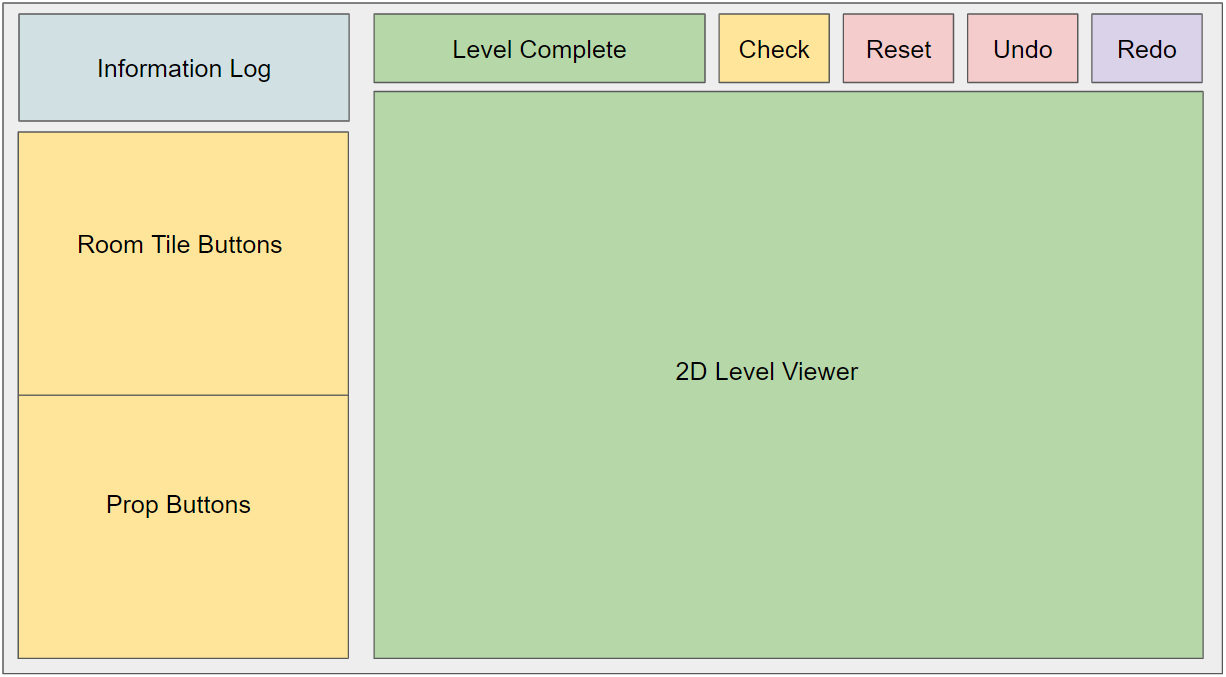
\includegraphics[width=1.0\linewidth]{LevelEditorLayout.PNG}
	\caption{The first iteration of the proposed level editor}
	\label{myLevelEditor}
\end{figure} 

\subsection{Level Editor Design}
In this experiment, there were two kinds of game objects that can be placed in the level rooms and props. Rooms occupy tiles on the map, whereas the props can be placed within any of the rooms. Figure~\ref{myLevelEditor} shows the first prototype design for the level editor. Barnes \textit{et al}\cite{barnes2015designing} suggests that any MI component should provide the reasoning behind the agents' actions, to do this the design contains an information log. The information log informs the participants why the level editor has made a particular decision. The level view is a tile-based view of the current map, it allows users to place tiles and props according to their respective rules. Figure~\ref{myLevelEditor} also shows the layout of the level editor, on the left is where the buttons to switch between what props/rooms are placed when the participant next clicks. There is a checking algorithm that makes sure there are a start and an end tile, it also checks these tiles are connected by a valid path. The level complete button executes this checking algorithm before finishing to make sure a valid level is being submitted. When the checking algorithm returns a false, the information log informs the user why it has been rejected.

\subsection{Prediction Technique}
When deciding the prediction technique for this experiment the main limiting factor to consider is the number of data points available. In the MI level editors discussed in Section~\ref{UI},  the number of tiles presents within a level did not exceed 144 \cite{alvarez2018fostering, liapis2013sentient, baldwin2017mixed}. By treating each tile as one data point this gives a maximum number of 144 data points to use when training the MI component. It has been proven that CBR techniques are effective, even with a small data set \cite{shepperd2001comparing,wen2012systematic}. However, SWR has been proven to outperform CBR on multiple occasions \cite{shepperd2001comparing, schroeder2016understanding}. The application of SWR does not seem possible in the multivariable system presented in this level editor, instead, CBR was used to provide the probabilities for a type of prop to be in a given tile. These probabilities were then roulette sampled to produce the props that will actually be placed in the tile.  

\section{Software Development}
The front end of the level editor was written in HTML which provided the web nodes, CSS which provided styling for the web nodes and JavaScript with Canvas as the rendering API. The front-end logic and AI components were also written in JavaScript. All of the front end development was written using the WebStorm IDE, with Google Chrome to run and debug the application. Writing the application in the form of a website made the experiment easy to share which reduced the friction gathering results can create. It also reduced the chances of investigator/observer bias \cite{phillips1999double} to occur. The questionnaires that were asked after the creation of each level were embedded in the application to provide a complete and contained experiment. Git was used as the version control software, with the repository for the Git project hosted on Digital Ocean server. On the server side, a Git post-commit hook was set up to automatically deploy any changes in the master branch to the website. The server code that handles the processing of the data sent to the server is written in python3 using the HTTP server module. Python3 was used because it was easy to set up and the run time performance of the application was not a priority. The Python3 module called TinyDB was used for the databasing API. TinyDB does not scale well but as this was a small experiment, the convenient way TinyDB stores data outweighs the performance losses. 

\subsection{System Development Life cycle}
The development of the application used for this experiment was undertaken by only one person. The level designer can be used to create levels for the game called "What is that Meat?", however, there are no dependencies between the two systems. This meant the application of a life cycle method such as Agile Development which focuses a lot on team dynamics and communication\cite{agile} would be less applicable to this kind of solo project. For this project, the incremental Model was used. The incremental model is made of phases, where at the end of each phase the product is given to the users. The feedback from the users is used in the creation of the next product, or increment \cite{massey2012comparing}. An incremental model approach is appropriate to use when the full requirements of a system are not known as it gives development flexibility \cite{isaias2015information}. 

The first phase (increment) of the application had all of the features and layout as shown in Figure~\ref{myLevelEditor}. The application was then given to a pilot group of three users. All of the sessions in this small group were supervised so that quality could be assured first hand. In the first increment of the application, the AI would only place props when it already had a history of what props to place in that room. The placing of the props would only happen when a new room was placed. Through observation, it was noted that users tended towards placing all of the rooms for a level first and then filling the rooms with props. This meant the prop placement part of the MI tool was not being used. 

The observations and feedback from the first phase were used to fuel the second phase of development. The lack of engagement with the prop placer was solved by a system that showed the user the props that the MI wants to place in the existing rooms. When the users are placing props in a room, low opacity props are placed in other rooms to indicate what props the MI tool wants to place. Another button was added to the toolbar which places all of the MI suggested props. Figure~\ref{levelEditorFinal} is a screenshot of the final application, along the top bar the Prop Fill button can be seen. The Prop Refresh button can be used to change the seeds of the random number generator used to generate the props. These features are not available in the levels where the MI tool is disabled. Upon completion of this phase, the application was given to two experts in the fields of AI and game development for heuristic evaluation.  Cockton and Woolrych\cite{cockton2002sale} believe that heuristic evaluations do not encourage a comprehensive view of an interface. However, a heuristic evaluation performed early on the development process is good \cite{nielsen1990heuristic} and it is cheap in terms of resources \cite{nielsen1990heuristic}. From the evaluation, three main problems were identified.
\begin{itemize}
\item The mixed-initiative tool did not take into account the location relative to the room the props were placed.
\item The Make Paths should connect all rooms to a path that reaches the start and end tile.
\item There is no context for making the levels, or what the props mean.
\end{itemize}

The usability issues identified were once more fed back into the development cycle. The CBR algorithm was re-designed to take into account the relative position of the props in the room. The Make Paths button was extended to make paths from all of the rooms to a path that connected to the start and end rooms. To give the users context and insight into their design decisions a small turn-based game was created alongside the application. Adding a way for the users to playtest the games they make is crucial to making a great game \cite{winn2006resolving}. The game that was made is a simplified  2D version of the game "What is that Meat?". The participants can play test their level at any time provided the minimum requirements for the level have been met. The application was given to a pilot study of four users and was observed to check for usability issues. This increment of the application did not contain any problems and was considered ready to start the experiment.

\begin{figure}[h]
	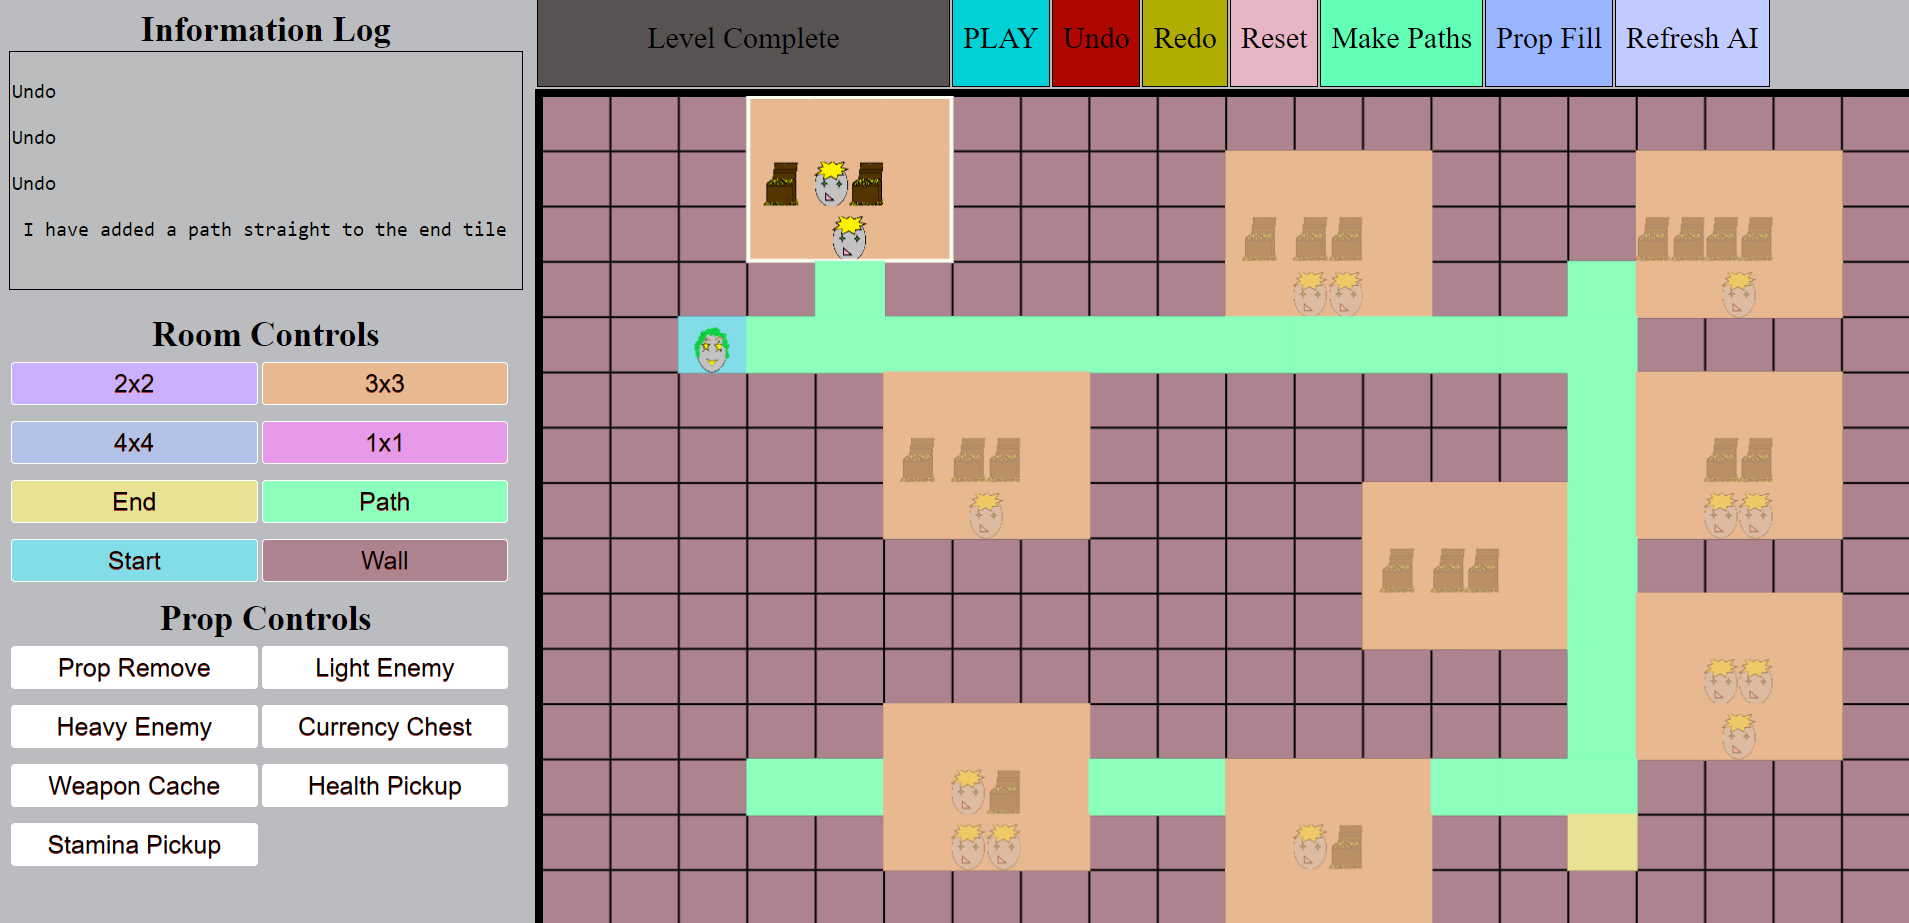
\includegraphics[width=1.0\linewidth]{LevelEditorFinal.PNG}
	\caption{The final view of the interface during a Mixed-Initiative level}
	\label{levelEditorFinal}
\end{figure} 

\subsection{Software Testing}
Unit testing was introduced early on in the life cycle of the application. Jest is a testing library for JavaScript applications run in the Node.js runtime environment. Jest was used in this experiment because it contained all of the features needed to create unit tests for this application. In addition, Jest has very good documentation and there are many good examples on GitHub.  To ensure a consistent styling throughout the application JSHint was used to perform checks on the applications source code. The tests for this application were integrated into the main project through the use of the library called pre-commit. Pre-commit is a  Node.js library which provides an easy way to integrate unit testing into Git using git hooks. Before any changes could be committed, all of the unit tests would need to pass and there must be no styling mistakes. If a test were to fail or a styling mistake identified the commit would not occur. 


\section{Results and Analysis}
The data from the experiment were processed in Python and was retrieved from the server using an HTTPS Post request. Three Python libraries were used to analyse the data. Scipy was used to provide the statistical functions, Numpy for more statistic functions and data handling and Matplotlib to generate the graphs. Python was used so that the graphs could also be generated when new data comes in. Each following subsection focuses on a different hypothesis and the results gathered to test that hypothesis. Some subsections contain additional results to provide greater context for the discussion.

\subsection{The MI component will affect the speed at which the participants create levels}\label{speedSec}
This hypothesis focused on the time it took for the participants to finish creating each level. The results showed a large distribution of times when all of the maps were combined into one list.  Figure~\ref{speedDoubleHist} shows the distribution of the maps with and without the MI component. Figure~\ref{speedDoubleHist} shows there is a cluster of times around the 100-300 second mark but both MI and no MI contain some maps that took much longer. The large distribution in time can be attributed to the differing work speeds of the individual participants. To reduce this the times were compared on a per user bases. A ratio of the time it took with the MI tool divided by the time without the MI was calculated for each user and added to a list. A \textit{t}-test produced a \textit{p}-value of 0.001254 and a \textit{T}-Value of 3.4381. The \textit{p}-value for this test is very low, which means for this experiment the null hypothesis can be rejected. The mean ratio of time was 1.636 which means that on average it took each user 1.636 times longer to create maps with the MI component. The Cohen's \textit{d} effect size was 0.9923. A Cohen's d effect size of greater than 0.8 would suggest a large effect size \cite{cohen1988statistical}.

\begin{figure}[h]
	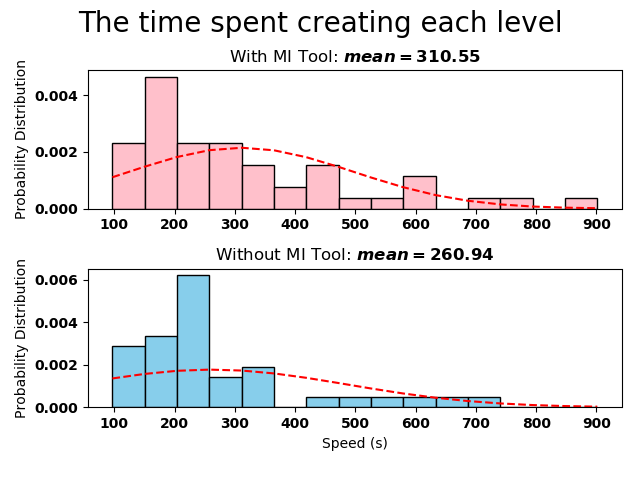
\includegraphics[width=1.0\linewidth]{Thetimespentcreatingeachlevel.png}
	\caption{Histogram of the time taken to create levels with and without the MI component}
	\label{speedDoubleHist}
\end{figure} 

\subsection{The MI component will affect the size of the levels the participants create}\label{sizeSec}
For this hypothesis, the two dependent variables used were the number of props and the number of tiles present in the level. There is a large distribution with the number of props and tiles. Figure~\ref{BoxObj} shows a box plot for the number of objects that were at each level. From Figure~\ref{BoxObj} there can be seen a general skew towards a larger number of objects with MI tool, than without. A ratio of the number of each object with divided by without the MI component was calculated. This removed the uncertainty created by comparing different participants design styles. Table~\ref{size} shows the values calculated from a \textit{t}-test on the list of ratios generated from the data. It would appear that the \textit{p}-value for both the ratios of props and tiles are significant as they are less than 0.05. Both the tiles and the props have roughly the same Effect sizes at 0.7, which suggests a large effect size\cite{cohen1988statistical}. It is interesting to note the large difference in means between the props and tiles. For every prop in a no MI level, there were two in an MI level. With tiles, there were 1.353 tiles in an MI level to everyone in a no MI level. Table~\ref{RemovedObjects} shows the percentage of MI placed objects that were removed by the participant, it shows that the participants removed about 50\% of all tiles placed by the MI and about 30\% of props.

The increase in objects could have been caused by the increase in time spent creating the level described in Section~\ref{speedSec}. However, a \textit{t}-test performed on the number ratio of props against the ratio of time it took to complete the level returned a \textit{p}-value of 0.4107 which is too high to show significance. A similar \textit{t}-test performed on the ratio of tiles against the ratio of time produced a \textit{p}-value of 0.2789 which once again is too high to prove a meaningful correlation.
\begin{figure}[h]
	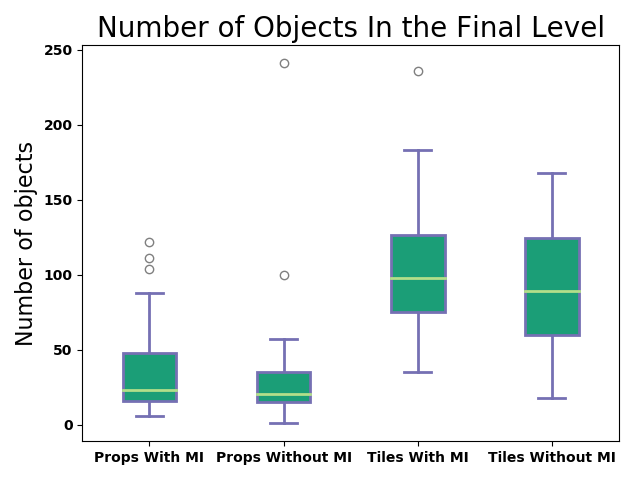
\includegraphics[width=1\linewidth]{NumberofObjectsIntheFinalLevel.png}
	\caption{Box plot of the number of objects in the final level}
	\label{BoxObj}
\end{figure} 

\begin{table}[h]
	\centering
	\caption{Number of Objects Values Table}
	\label{size}
	\def\arraystretch{2}
\resizebox{\columnwidth}{!}{\begin{tabular}{|l|l|l|l|l|}
		\hline
		\textbf{Object Type} & \textbf{\textit{P}-Value}& \textbf{\textit{T}-Value} & \textbf{Cohen's \textit{d} Effect Size}& \textbf{Mean Ratio MI/No MI}\\\hline
		Tiles &0.01457&2.539&0.7329&1.353\\ \hline
		Props &0.01570&2.509&0.7242&2.002\\ \hline

	\end{tabular}}
\end{table}

\begin{table}[h]
	\centering
	\caption{Percentage of Objects placed by the MI that were removed}
	\label{RemovedObjects}
	\def\arraystretch{2}
\resizebox{\columnwidth}{!}{\begin{tabular}{|p{4cm}|p{4cm}|}
		\hline
		\textbf{Tiles} & \textbf{Props}\\\hline
		47.48\% &28.86\%\\ \hline
	\end{tabular}}
\end{table}

\subsection{The MI component will affect the number of the clicks the designer makes}\label{clicks}
To test this hypothesis the number of clicks the user made in each level was recorded. The clicks with and without the MI component were calculated as a ratio on a per-user basis. A \textit{t}-test on the ratios produced a \textit{p}-value of 0.008758 and a \textit{T}-Value of 2.738. The Cohen's \textit{d} effect size was 0.7904 which would suggest a large effect size\cite{cohen1988statistical}. The mean click ratio was 1.622, which means that on average for every click done on a no MI level, 1.6 clicks were done on an MI level.  Figure~\ref{clickDist} shows several bins with a high number of clicks for MI enabled levels.

The average increase in clicks may be related to the size of the level. Section~\ref{sizeSec} describes that on average the levels with the MI component have twice as many props and 1.353 as many tiles than levels without the component. A \textit{t}-test performed on the ratio of clicks against the number of props returned a \textit{p}-value of 0.4133 and against tiles a \textit{p}-value of 0.3181. Both of the \textit{p}-values are too high to show a significant relationship between the number of clicks and the size of the level.

\begin{figure}[h]
	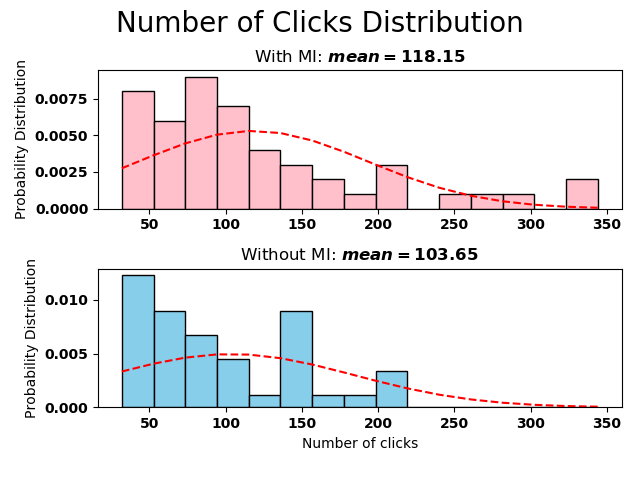
\includegraphics[width=1\linewidth]{NumberofClicksDistribution.png}
	\caption{Histogram of the number of clicks for each level}
	\label{clickDist}
\end{figure} 

\subsection{The MI component will influence participants to explore other level designs}\label{alter}
The dependent variable used to test this hypothesis came from the questionnaire response to the question "How frequently did the level editor make you consider an alternative level design?". A Mann-Whitney U \cite{mann1947test} test was used to determine the significance between the questionnaire response with the MI and the questionnaire response without the MI component. The Mann-Whitney U test was used as the questionnaire data is ordinal and the comparison is made between two independent groups (with MI and without MI).The test produced a \textit{p}-value of 0.02223 and a \textit{u}-value of 885.5. Cohen's \textit{d} effect size is 0.4311, which would suggest a medium effect size \cite{cohen1988statistical}. Figure~\ref{alterHisto} shows a double histogram containing the numerical representation of the questionnaire responses for both the MI levels against the no MI levels. Table~\ref{responsValues} displays how the responses correlated to the numbers shown on the histogram. The mean value of how often users were influenced to explore an alternative level design with the MI component is 1.813 without the MI component the value is 1.292. From the two means we can argue that when the MI component is active, participants found that the level editor challenged them to think about alternative level designs more often. Figure~\ref{alterHisto} shows that there are some participants that fell between the frequently - very frequently categories with the MI component. It also shows that there are were no participants that thought the level editor frequently to very frequently made them consider an alternative level design.  

\begin{figure}[h]
	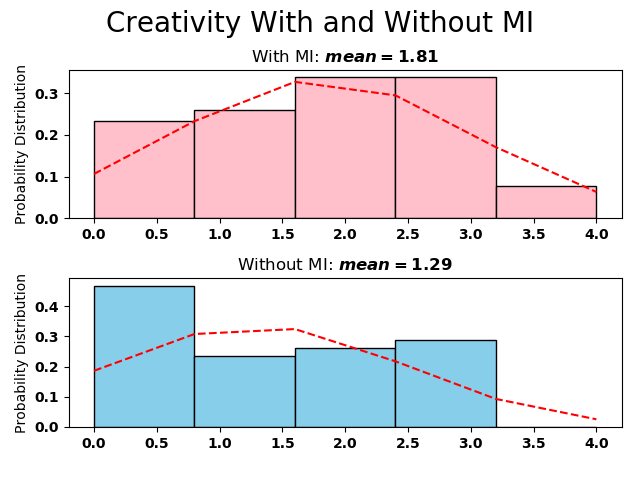
\includegraphics[width=1\linewidth]{CreativityWithandWithoutMI.png}
	\caption{Histogram of how often users were influenced to explore other level designs.}
	\label{alterHisto}
\end{figure}
\begin{table}[h]
	\centering
	\caption{Questionnaire Response Numerical Values}
	\label{responsValues}
	\def\arraystretch{2}
      \resizebox{\columnwidth}{!}{\begin{tabular}{|l|l|l|l|l|}
		\hline
		\textbf{Never} & \textbf{Rarely}& \textbf{Sometimes} & \textbf{Frequently}& \textbf{Very frequently}\\\hline
		0 &1&2&3&4\\ \hline
	\end{tabular}}
\end{table}

\subsection{The participants with more experience will be Negatively impacted more often by the MI component}
The two dependent variables tested for this hypothesis were both ordinal and from the questionnaire. The users were asked at the end of each level: "How difficult did you find it to make the level you wanted?", the responses ranged from very hard to very easy. A Spearman's correlation was used to test the correlation between the users' experience and how difficult they found it to create the levels with the MI component. A Spearman's correlation is recommended to use when dealing with data that is not normally-distributed\cite{o2005step}. The output from a Spearman's correlation on the two variables produced a \textit{p}-value of  0.4196, which is above 0.05 so the null hypothesis cannot be rejected. 

\section{Discussion}
The results in this experiment show that an MI component can have a clear impact on the levels created by a designer. It is hard to label the net impact of the tool as either positive or negative. In this section, the potential implications of each hypothesis will be discussed.  

\subsection{The MI implementation}\label{implementation}
 The implementation of the MI component plays a large part in the way the participants interacted with it. In this level editor, the MI component could make pivotal design decisions such as the pathways between each room. Table~\ref{RemovedObjects} shows that the participants often removed the pathways the MI component placed. The layout of the map and how the rooms connect together could be seen as an abstract concept. Barnes \textit{et al}\cite{barnes2015designing} found that human designers were better at making abstract decisions and inferring meaning than an AI agent. It could be argued the results shown in table~\ref{RemovedObjects} support Barnes \textit{et al}\cite{barnes2015designing} findings as the high percentage of removed MI decisions could mean the MI does not understand the abstract idea for the map. 

\subsection{The MI component will affect the speed at which the participants create levels}\label{speedDiss}
Section~\ref{speedSec} shows, at a significance level of 0.1\%, that when the MI tool is present the time the users spend on each level increases. These results would suggest that adding an MI component to a level editor would not be effective for the prototyping phase, as prototypes are meant to be quick and easy to produce \cite{budde1992prototyping}. One cause for this increase in time could have been caused by the time it took to remove decisions made by the MI component. Section~\ref{implementation} describes how giving the MI component the ability to make pathways may have caused the MI component to make suggestions that did not align with the ideas of the designer. This misalignment of the MI components vision for the level and the designers could have been the cause for the increase in time. 

The results found in section~\ref{speedSec} indicated that the increase in speed found in predictive texting by Dunlop and Crossan\cite{dunlop2000predictive}, may not apply to level design. However, the way in which users were tested in Dunlop and Crossan\cite{dunlop2000predictive} differs from how the participants were tested in this paper. In this experiment, participants were not given a number of objects in the scene they had to place, instead, they were allowed to place as many as they wanted. This added some uncertainty as it meant participants could make levels as big as they wanted to. 

\subsection{The MI component will affect the size of the levels the participants create}
Section~\ref{sizeSec} describes how the mean ratio for both the number of tiles and props is greater than one and both stats are significant to a level of 2\%.  The results show ratios of above one, which suggests that the MI component did increase the size of the levels, similar to results found by Ling \cite{ling2005length} with predictive texting. It could be argued that the increase in the size of the levels is related to the increase in the time it took for participants to create the levels. Section~\ref{sizeSec} includes the results of a \textit{t}-test looking for a relationship between the size of the MI levels and the time it took to create the levels. The results from the \textit{t}-test did not show a sign below the 5\% level. This would suggest the increase in the size of the level did not come from the extra time spent with the MI levels, but instead from the interaction with the MI. In this experiment using the MI component, on average, doubled the number of smaller objects placed in the level. This would suggest if the map the designer is trying to prototype should have lots of small objects, it may be beneficial to include an MI component to handle the placement of these objects. 

\subsection{The MI component will affect the number of the clicks the designer makes}
The results described in section~\ref{clicks} would suggest the addition of the MI component to a level editor increases the number of clicks the users have to make. It can be argued that adding an MI component to a level editor did not solve the feature requested by one of the participants in the paper written by Alverezs \textit{et al}\cite{alvarez2018fostering}. One cause for the increase in the number of clicks could have been the implementation of the MI component. As discussed in section~\ref{implementation}, the removal of the objects placed by the MI component could have caused an increase in clicks. 

\subsection{The MI component will influence participants to explore other level designs}\label{altDiss}
Arguably, the main purpose of prototype levels is to explore potential ideas. These data described in section~\ref{alter} suggests that having an MI component that works alongside a designer, may make them consider an alternative level design. These results also support the findings of Alverezs' \textit{et al}\cite{alvarez2018fostering}. It can be argued that influencing participants to consider alternatives is a great aid during the design process. Even if the ideas presented by the MI are not accepted by the user, they have still considered search spaces that would otherwise have remained unexplored. This would suggest adding an MI component to a level editor may increase the variety of levels produced by the designers.

The participants also found the level editor influenced them to explore other level designs without the MI component present. This could have been caused by the level editor not allowing them to submit a map that cannot be completed. It can be argued that giving the level editor the ability to tell which maps are completable is a form of intelligence. This would mean, even without the extra tools provided by the MI component, the level editor could still be considered an MI tool. 

\subsection{The participants with more experience will be Negatively impacted more often by the MI component}
In this experiment, there were no significant results to suggest that the users level design experience affected the way they interacted with the MI component. For all participants in the experiment, it was there first time interacting with the level editor. Regardless of experience all of the users were using a new tool for the first time. This meant the participants had no expectations of what that tool should or could do. This could be why there were no significant results to suggest the users with more experience were negatively impacted by the tool.

\section{Future Work}
One unanticipated result is how frequently the MI placed tiles were removed. Section~\ref{implementation} describes reasons to why the MI placed pathways were removed so often. The argument presented in Section~\ref{implementation} could have affected all of the hypothesis tested in this experiment. Further work should be done to see what effects reducing the MI components ability to make decisions may have.

In section~\ref{speedDiss} this paper argues that adding an MI system may increase the time it takes for users to complete levels. The original work by Dunlop and Crossan\cite{dunlop2000predictive} that motivated this hypothesis took a very different approach to measure the speed the user created levels. Dunlop and Crossan\cite{dunlop2000predictive} set out a specific goal for the users to type and timed how long it took to achieve that goal. In this paper, to test the speed, the users could finish the level once they had placed a minimum number of objects. They could keep going for as long as they wanted. To make the results more comparable to the results found by Dunlop and Crossan\cite{dunlop2000predictive} further work should be done that requires the user to place exactly a specified number of objects and time that instead.

The results and discussion presented in section~\ref{altDiss} seem to affirm the findings of Alverezs' \textit{et al}\cite{alvarez2018fostering}. However, in this experiment all of the results in this area are based on one questionnaire response. Further work should be done, to explore the accuracy of the findings in Alverezs' \textit{et al}\cite{alvarez2018fostering} and the findings present in this paper. Additional research could include a questionnaire which is more comprehensive as well as a more refined novelty search algorithm.

In this experiment, CBR was used in the prediction algorithm. SWR could not easily be adapted to fit with the data structures present in the level editor. If SWR could be modified to work in the context of this level editor, the existing research suggests that it would provide better predictions \cite{shepperd2001comparing, schroeder2016understanding}. More research should be done to measure how the prediction methods use may change the way users interact with the level editor. 

\section{Conclusion}
Existing literature in the field of MI level design focuses on how an MI component can help with the creative process. The focus of this paper was the effect that adding an MI component may have the level design process. The results in this paper give insight into the kind of effects integrating an MI system into a level editor may have. This paper has argued that integrating an MI component into a level editor will affect both the designer and the levels created by the designer.

This study found four significant effects that adding an MI component may have. 
These effects are: 
\begin{itemize}
\item An increase in the size of the levels create.
\item An increase in the time it takes to create each level.
\item An increase in the number of clicks participants has to make.
\item An increase in the exploration of alternative level designs.
\end{itemize}

When one is planning on integrating an MI system into the level design process, much thought should be put into the MI responsibilities. In this paper, a system was created that could make large scale decisions. These decisions were often not kept by the participants. In the creative endeavour that is level design, perhaps MI systems should not be allowed to make large decisions. As discussed in section~\ref{implementation}, the implementation of the MI system plays the largest part on the kind of effects it may have. This paper recommends planning carefully the type and scale of the decisions the MI can make. This paper has shown, that users are much more willing to accept the help implementing the finer details, than the larger picture.

\bibliographystyle{IEEEtran}
\bibliography{references}

% Appendices
\appendices
\section{Acknowledgements}
I would like to thank all of the staff at Falmouth University for their support and guidance. I would also like to thank my dissertation supervisor Ed Powley. My thanks go to my classmates for the help provided in the peer reviews sessions.

\section{Reflective Report}
Each of the following subsections pertains to a different problem encountered during this dissertation. The subsections each include a SMART goal that addresses the problem raised in that section.

\subsection{The level editor}
From a visual perspective, the quality of the interface leaves a lot to be desired. I was informed by some participants that it was hard to really understand the context of the editor due to poor visuals. I understand the potential for this misunderstanding to have affected the results produced by the interface. To improve this I would create a colour coded system for all of the props to group them into the functions they serve. For example, all of the enemies would have red elements, to represent danger. I could measure the effectiveness of the colour coding by performing a small pilot study on different colour groupings, picking the most effective. I believe colour coding may make it easier to understand the interface. Doing this before the main experiment would be the most effective time. 

\subsection{Prediction algorithm}
From the literature review, the SWR procedure seemed to yield the most accurate predictions. However, I could not fit the SWR procedure to my project. I believe switching to CBR may have caused a significant loss in accuracy. To determine whether or not SWR would have made a difference I could try and implement SWR in the level editor again and do a \textit{t}-test comparing how often users removed objects. The \textit{t}-test results should give me a good measure of what kind of effect not using SWR may have had. This would require another round of study, but the only additional programming would be trying to fit SWR into the level editor. I think it would be useful to do this experiment before any other experiments done in this level editor.

\subsection{Speed test}
I think the design of the experiment used to test the speed at which the users created the levels was somewhat flawed. I do believe the results gathered are relevant and do have meaning to the field. However,  I do not believe they accurately test the predictive texting findings from which the hypothesis is drawn. To accurately test the seed of predictive texting findings I should have asked the participants to create levels of an exact size and timed how long it took for them to do that. I could measure the effectiveness of this alternative experiment design by seeing how the results from the new experiment differ from the current results. I would have to be careful using this as a unit of measurement as it may cause bias in the experiment. Changing the programming of the experiment should not be difficult and could be done quite quickly.

\subsection{Play testing}\label{ptest}
Giving the participants the option to playtest the levels they created came about halfway through the development of the artefact. It came from the need to give the participants context in regards to the levels they were creating. I debated for some time whether or not to include the time spent playtesting in the total time for the level. After getting feedback from some of the design lecturers I concluded that playtesting a level is an integral part of level design, and certainly should be counted in the total time to make a level. Unfortunately, I believe may have created a lot of noise in the data sets. To see how much of an impact this may have made I think it would be good to do a test with and without the ability to playtest the levels. By comparing the distributions of the test with and without the playtest feature, this will give a good measurement to the amount of noise generated by the feature. This may mean the participants lose context on the levels they are creating, but it may reduce some of the noise. This should be done before any more time-based experiments are done with the editor, as the results may impact those times greatly.

\subsection{Tutorial}
The tutorial I created contained all of the knowledge required to use all of the features the level editor had. I tracked whether or not the participants did the tutorial or not. Every participant did complete the tutorial, which consisted of several windows with a GIF and a brief description. Looking back, I believe it would have been more effective to make an interactive tutorial which forced the participants to use every feature at least once. Currently, there were some participants who didn't use some features of the level editor. I think the interactive tutorial will be more effective as it would be engaging and interesting. To improve future work, creating a better tutorial should ensure the users have a better knowledge of the system they are using. An AB test could be done to measure how effective the interactive style of the tutorial is. By doing this, I would know what tutorial style works best for this level editor. 

\subsection{Conclusion}
In conclusion, I believe the research project I have undertaken does add knowledge to the field of MI level editors and, to a lesser degree, the field of MI systems. There are some areas where more careful planning and the mirroring of existing literature may have produced a better outcome. Despite this, I am proud of the literature I have authored and the complex programming artefact I have created.

% that's all folks
\end{document}
